%----------------------------------------
% Preamble to set up the document
%----------------------------------------
\documentclass{article}

% set up packages (you shouldn't need to touch this)
\usepackage{graphicx}  % required to insert images
\usepackage{hyperref}  % for hyperlinks
\usepackage[svgnames]{xcolor}  % to change hyperlink colors
\colorlet{linkcolour}{DarkBlue}
\hypersetup{colorlinks=true, linkcolor=linkcolour, citecolor=linkcolour, urlcolor=linkcolour,}

% Margins
\topmargin=-0.45in
\evensidemargin=0in
\oddsidemargin=0in
\textwidth=6.5in
\textheight=9.0in
\headsep=0.25in

% use a sans serif font
\renewcommand{\familydefault}{\sfdefault}

%----------------------------------------
% Step 1: Edit the lecture title
%----------------------------------------
\title{
Lecture 9: Classification: Naive Bayes\\  % Lecture title
Modeling Social Data, Spring 2019 \\   % Course title
Columbia University                    % School
}

%----------------------------------------
% Step 2: Edit your name and the date
%----------------------------------------
\author{Jiayi Lily Ma}                     % Scribe's name
\date{March 29, 2019}                % Lecture date

\begin{document}

\maketitle


%----------------------------------------
% Step 3:
% Rename uni.tex to match your uni,
% edit the filename accordingly below,
% and put your notes in this file
%----------------------------------------
%----------------------------------------
% Write your notes here
%----------------------------------------

\section{Learning by example}
Spam vs Ham
\begin{description}
  \item[$\bullet$] We can separate spam from non-spam emails by looking at various indicative things 
  \item[$\bullet$] For example, words such as 'special offer' are highly indicative of spam, whereas words like 'supercomputing cluster' are much less indicative. 
  \item[$\bullet$] A potential problem is with ubiquitous words like 'the'.
  \item[$\bullet$] It's hard to write down all rules, so we learn them from data instead. 
\end{description}

\section{Diagnoses a la Bayes}
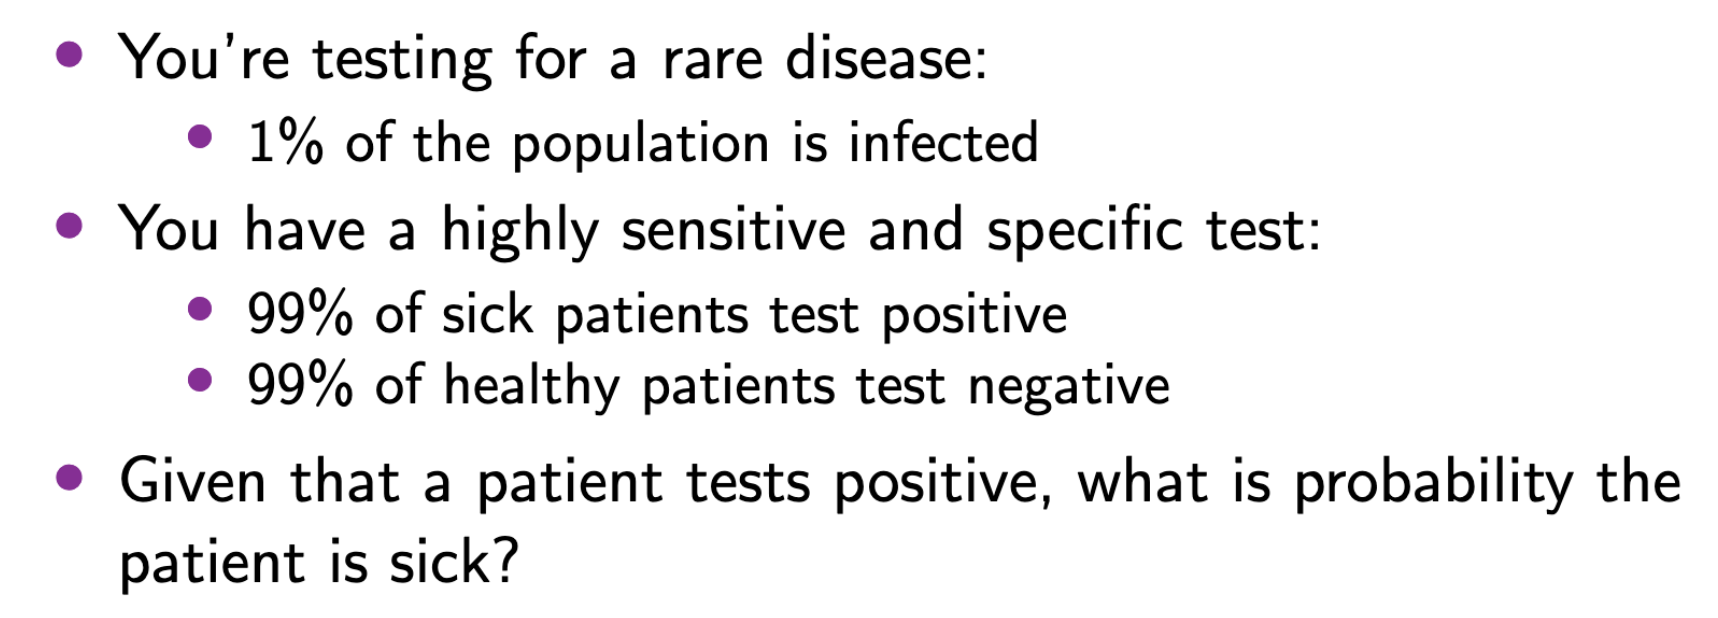
\includegraphics[width=100mm, scale=0.5]{figures/bayes.png}

\subsection{Method 1}
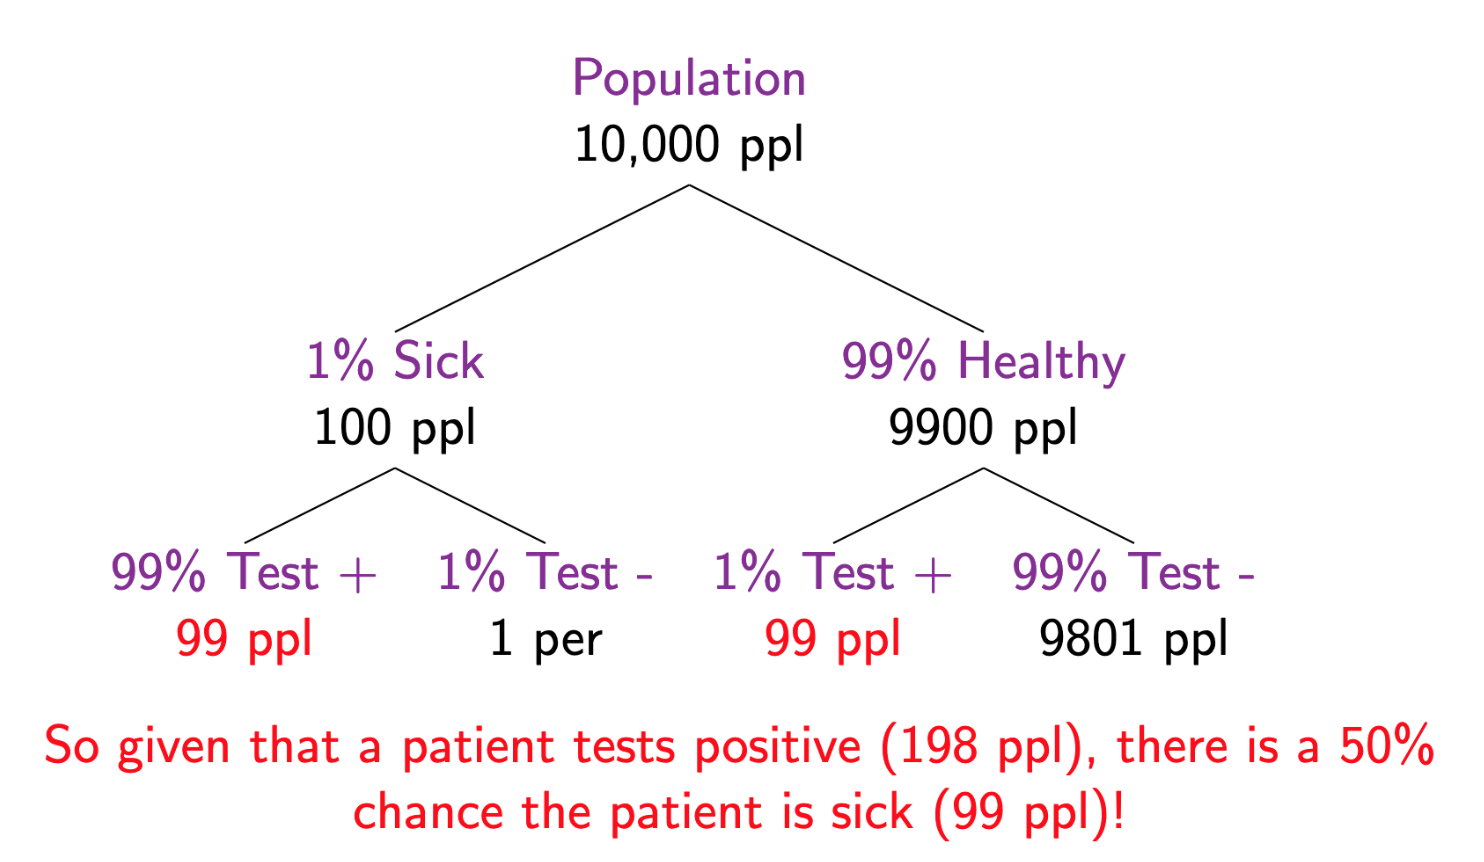
\includegraphics[width=100mm, scale=0.5]{figures/tree.png}

\subsection{Method 2}
We know from the given that: 
$$P(sick) = 0.01$$
$$P(healthy) = 0.99$$
$$P(+ | sick) = 0.99$$
$$P(+ | healthy) = 0.01$$

According to Bayes' Theorem (proven later):
$$
P(sick | + ) = \frac{P(+ | sick)P(sick)}{P(+)} 
= \frac{P(+|sick)P(sick)}{P(sick)P(+|sick) + P(healthy)P(+|healthy)}  = 
\frac{(0.99)(0.01)}{(0.01)(0.99)+(0.99)(0.01)} =
\frac{1}{2}
$$

\section{Natural Frequencies a la Gigenrenzer}

\begin{description}
\item[$\bullet$]Compared to the 1000 women who didn't have screening, the 1000 women with screening suffered 100 cases of false-positive negative results and 5 cases of unnecessary treatments. 
\item[$\bullet$] Thus, although the claim is that screening reduces the number of patients who died from breast cancer by 20\% (5 deaths vs 4 deaths), there's a risk present for error for women with screening that is not present for those without.
\end{description}


\section{Inverting Conditional Probabilities}
Bayes' Theorem

We know that
$$P(x,y) = P(x|y)P(y) = P(y|x)P(x)$$ because $P(x,y) = P(y,x)$

Divide to get the probability of y given x from the probability of x given y:
$$P(y|x) = \frac{P(x|y)P(y)}{P(x)}$$ where $P(x) = \sum_{y \in \Omega_Y}P(x|y)P(y)$

\section{(Super) Naive Bayes}
Idea: use Bayes' Rule to build a one-word spam classifier:

$$P(spam|word) = \frac{P(word|spam)P(spam)}{P(word)}$$

Estimate each term with ratio of counts: 

$$\hat{P}(word|spam) = \frac{
\textup{\# 
spam docs containing word}}{\textup{\# spam docs}}$$
$$\hat{P}(word|ham) = \frac{\textup{\# ham docs containing word}}{\textup{\# ham docs}}$$
$$\hat{P}(spam) = \frac{\textup{\# spam docs}}{\textup{\# docs}} $$
$$\hat{P}(ham) = \frac{\textup{\# ham docs}}{\textup{\# docs}}$$

Examples from running bash script: \\

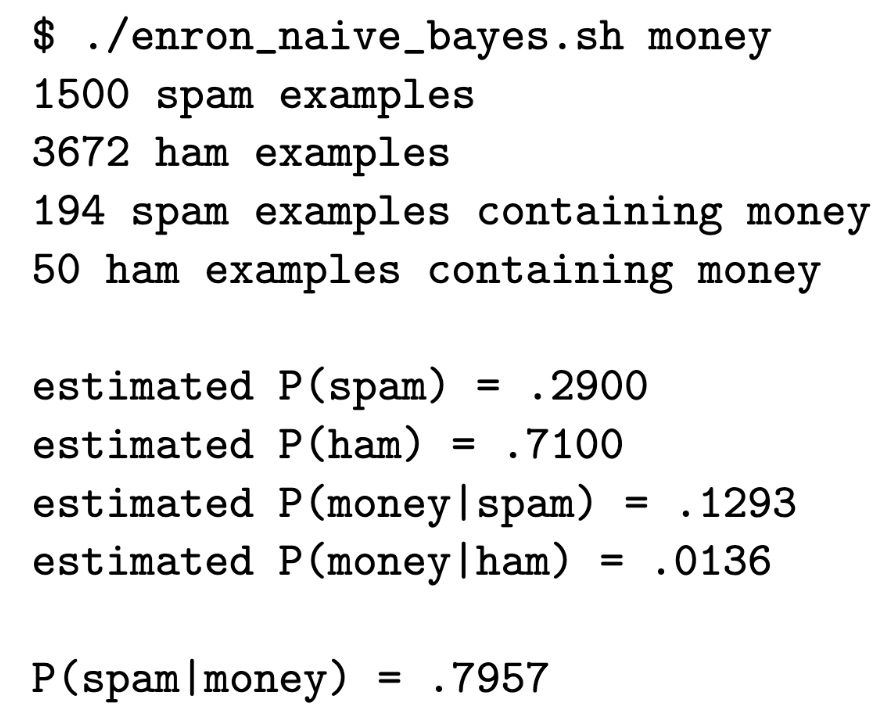
\includegraphics[width=100mm, scale=0.5]{figures/ex1.png}\\
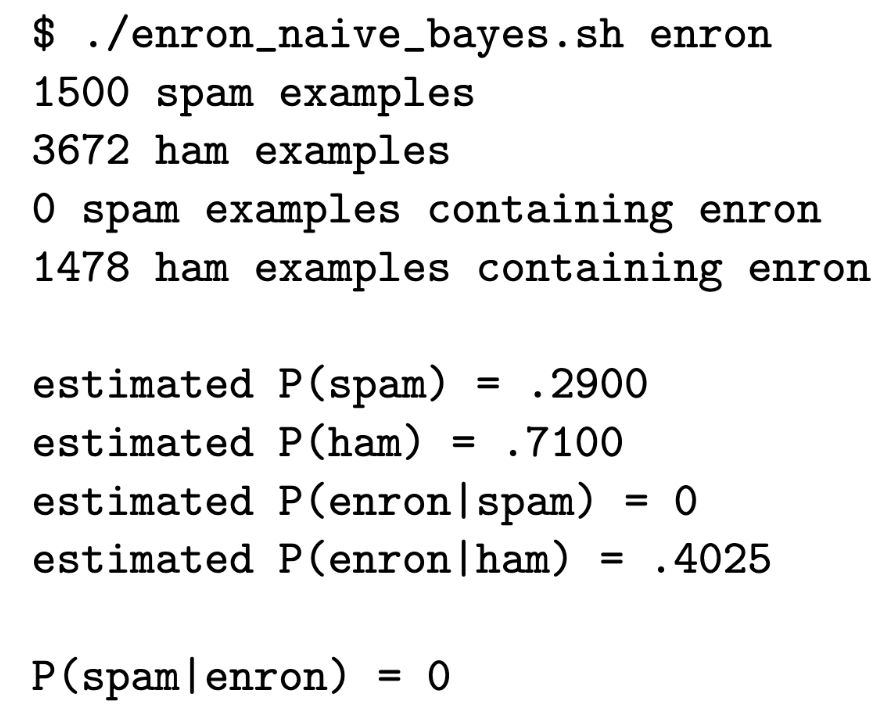
\includegraphics[width=100mm, scale=0.5]{figures/ex2.png}\\

Note that the probability of an email with the word 'enron' being classified as spam is 0 because none of the spam examples has 'enron'. This is probably not what we want. 

A possible way around this is: 

$$\hat{P}(word | spam) = \frac{n_{word, spam} + \alpha }{N_{spam} + \beta}$$

where the best $\alpha$, $\beta$ combination on the test data can be found through grid search.

\section{Naive Bayes}
\begin{description}
\item[$\bullet$] 'Naive' in the sense that all words in a document are seen as independent given the class label of the document.
\item[$\bullet$] Represent each document by a binary vector $\Vec{x}$ where $x_j = 1$ if the j-th word appears in the document ($x_j = 0$ otherwise).

\item[$\bullet$]If we model each words as \textit{independent} Bernoulli random variable, the probability of observing document $\vec{x}$ of class $c$ is: 

$$P(\vec{x}|c) = \prod_i\theta_{jc}^{x_j}(1 - \theta_{jc})^{1-x_j}$$

where $\theta_{jc}$ is the probability that the j-th word occurs in a document of class $c$.

\item[$\bullet$] Using this likelihood in Bayes' Rule and taking the logarithm, we have: 
\end{description}

$$ log P(c|\vec{x}) = log \frac{P(\vec{x}|c)P(c)}{P(\vec{x})} =  \sum_j x_j log(\frac{\theta_{jc}}{1-\theta_{jc}}) + \sum_j log (1-\theta_{jc}) + log \frac{\theta_c}{P(\vec{x})}$$

where $\theta_{j}$ is the probability of observing a document of class $c$ and $log P(\vec{x}|c)$ is calculated as follows: 

$$
    log P(\vec{x}|c) = \sum_j log[\theta_{jc}^x_j(1-\theta_{jc})^{1-x_j}] =  
    \sum_j{x_jlog\theta_{jc} + (1-x_j)log(1-\theta_{jc})}
    =
    \sum_j x_j log(\frac{\theta_{jc}}{1-\theta_{jc}}) + \sum_j log (1-\theta_{jc})
$$
Note that the second term $\sum_j log (1-\theta_{jc}$ is a constant because it doesn't depend on $\vec{x}$. It can be interpreted as the base rate of class $c$ for an empty document. Recall that $\theta_{jc}$ is the probability that the j-th word occurs in a document of class $c$. 

We can remove $P(\vec{x})$ by calculating the log-odds: 

$$log \frac{P(1 | \vec{x})}{P(0|\vec{x})} 
= \sum_j
x_j \underbrace{log\frac{\theta_{j1}(1-\theta_{j0})}{\theta_{j0}(1-\theta_{j1})}}_\text{w_j} + \underbrace{\sum_j log \frac{1-\theta_{j1}}{1-\theta_{j0}}+ log \frac{\theta_1}{\theta_0}}_\text{w_0}$$

which gives a linear classifier of the form $\vec{w} \cdot \vec{x} + w_0$

We train by counting words and documents within classes to estimate $\theta_{jc}$ and $\theta_c$: 

$$\hat{\theta}_{jc} = \frac{n_{jc}}{n_c}$$

$$\hat{\theta}_c = \frac{n_c}{n}$$ and then calculate the weights $\hat{w}_j$ and bias $\hat{w}_0$: 

$$\hat{w}_j = log \frac{\hat{\theta}_{j1}(1-\hat{\theta}_{j0})}{\hat{\theta}_{j0}(1-\hat{\theta}_{j1})}$$

$$\hat{w}_0 = \sum_j log \frac{1-\hat{\theta}_{j1}}{1-\hat{\theta}_{j0}} + log \frac{\hat{\theta}_1}{\hat{\theta}_0}$$

We predict by adding the weights of the words that appear in the document to the bias term. 

\section{Logistic Regression}
Form of classifier: 

$$ log \frac{p}{1-p} = \vec{w} \cdot \vec{x}$$

Solve for $p$: 

$$ \frac{p}{1-p} = e^{\vec{w}\cdot\vec{x}}$$ 
$$ p = (1-p)e^{\vec{w} \cdot \vec{x}}$$
$$p(1+e^{\vec{w} \cdot \vec{x}}) = e^{\vec{w} \cdot \vec{x}}$$

$$p = \frac{e^{\vec{w} \cdot \vec{x}}}{1+e^{\vec{w} \cdot \vec{x}}} \cdot \frac{e^{-\vec{w} \cdot \vec{x}}}{e^{-\vec{w} \cdot \vec{x}}} = \frac{1}{1+e^{-\vec{w} \cdot \vec{x}}} = P(\vec{x} | \vec{w})$$

The probability of seeing data $(\vec{x}_i, y_i)$ is: 

$$L = \prod_i p_i^{y_i}(1-p_i)^{1-y_i}$$

Note that $y_i \in {0,1}$ and $p_i = P(\vec{x_i}|\vec{w})$. \\

Take the log of $L$: 
$$ \ell = log L = \sum_i{y_i log (p_i) + (1-y_i)log(1-p_i)} = \sum_i{y_i log \frac{p_i}{1-p_i} + log(1-p_i}) = \sum_i{y_i(\vec{w}\cdot\vec{x_i}) - log(1+e^{\vec{x}\cdot\vec{x_i}})}$$

Note that $log(1-p_i) = log(1-\frac{1}{1+e^{-\vec{w}\cdot\vec{x}}}) = log(\frac{1}{1+e^{\vec{w}\cdot\vec{x}}}) = -log(1+e^{\vec{w}\cdot\vec{x}})$.\\

We want to find the $\vec{w}$ that gives the highest likelihood to the data that we have i.e. the $\vec{w}$ that maximizes $P(D|\vec{w})$. This is equivalent to finding a $\vec{w}$ that maximizes $log P(D|\vec{w})$. Note that this log probability is $\ell$, what we found previously. So we take the derivative of $\ell$ with respect to $\vec{w}$:

$$\frac{d\ell}{dw_j} =  \sum_j{y_ix_{ij} - \frac{1}{1+e^{\vec{w}\cdot\vec{x}_i}}e^{\vec{w}\cdot\vec{x}_i}x_{ij}} = \sum_j{y_ix_{ij} - p_ix_{ij}} = 
\sum_j (y_i-p_i)x_{ij}$$

note that $p_i = \frac{1}{1+e^{\vec{w}\cdot\vec{x}_i}}e^{\vec{w}\cdot\vec{x}_i}$ (see previous calculation).

We use this gradient in gradient descent to find the best $\vec{w}$. 

\begin{description}
\item[$\bullet$] Naive Bayes gives extreme estimates because it doesn't take the weight of other words into account. 
\item[$\bullet$] Logistic Regression, however, allows for the sharing of weights because $p_i$ is calculated with $\vec{w}$.
\end{description}





\end{document}

%%% Local Variables:
%%% mode: latex
%%% TeX-master: t
%%% End:
